\documentclass[border=5mm,tikz]{standalone}
\usepackage{pgfplots}
\pgfplotsset{compat=1.17}

\begin{document}

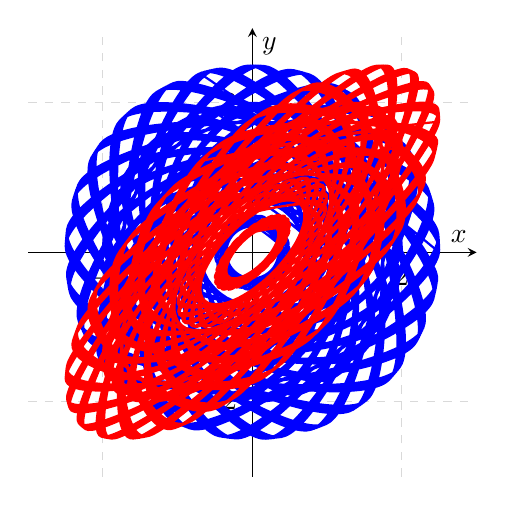
\begin{tikzpicture}
    \begin{axis}[
        xmin=-3, xmax=3,
        ymin=-3, ymax=3,
        axis lines=center,
        unit vector ratio*=1 1 1,
        xlabel=$x$, ylabel=$y$,
        grid=major,
        grid style={dashed,gray!30},
    ]

    % Original concentric circles
    \foreach \r in {0.5,1,...,2.5} {
        \addplot[blue,domain=0:360,samples=180,smooth, thick] ({\r*cos(deg(x))},{\r*sin(deg(x))});
    }

    % Transformed concentric circles
    \def\rho{0.7} % Set your desired value for \rho here, within [-1,1]
    \foreach \r in {0.5,1,...,2.5} {
        \addplot[red,domain=0:360,samples=180,smooth, thick] ({\r*cos(deg(x))},{\rho*\r*cos(deg(x)) + \r*sqrt(1-\rho*\rho)*sin(deg(x))});
    }

    \end{axis}
\end{tikzpicture}

\end{document}
